%%%%%%%%%%%%%%%%%%%%%%%%%%%%%%%%%%%%%%%%%%%%%%%%%%%%%%%%%%%%%%%%%%%%%%%%%%%%%%%
%%%%%%%%%%%%%%%%%%%%%%%%%%%%%%%%%%%%%%%%%%%%%%%%%%%%%%%%%%%%%%%%%%%%%%%%%%%%%%%
%%%%%%%%%%%%%%%%%%%%%%%%%%%%%%%%%%%%%%%%%%%%%%%%%%%%%%%%%%%%%%%%%%%%%%%%%%%%%%%
\RequirePackage[l2tabu, orthodox]{nag}
\documentclass[11pt,a4paper]{jarticle}
\usepackage[all, warning]{onlyamsmath}

%%%%%%%%%%%%%%%%%%%%%%%%%%%%%%%%%%%%%%%%%%%%%%%%%%%%%%%%%%%%%%%%%%%%%%%%%%%%%%%
%% packages 
\usepackage{amsmath}
\usepackage{amsfonts}
\usepackage{bm}
\usepackage{txfonts}
\usepackage{fancyhdr}
\usepackage{lastpage}
\usepackage{array}
\usepackage{multirow}
\usepackage{enumitem}
\usepackage{setspace}
\usepackage{boites}
\usepackage{cite}
%%%%\usepackage{udline}
\usepackage[hang,small,bf]{caption}
\usepackage[subrefformat=parens]{subcaption}\captionsetup{compatibility=false}
\usepackage[dvipdfmx]{color}
\usepackage[dvipdfmx]{graphicx} %% must be placed at the last line of ``\usepackage''s


%%%%%%%%%%%%%%%%%%%%%%%%%%%%%%%%%%%%%%%%%%%%%%%%%%%%%%%%%%%%%%%%%%%%%%%%%%%%%%%
%% margin
\setlength{\hoffset}{-1in}%
\setlength{\voffset}{-1in}%
\setlength{\oddsidemargin}{20truemm}%
\setlength{\evensidemargin}{20truemm}%
\setlength{\topmargin}{20truemm}
\setlength{\headheight}{5truemm}
\setlength{\headsep}{0truemm}
\setlength{\textheight}{250truemm}%
\setlength{\textwidth}{170truemm}%
\setlength{\marginparsep}{0truemm}
\setlength{\marginparwidth}{0truemm}
\setlength{\footskip}{4truemm}
%\setlength{\columnsep}{10truemm}

%%%%%%%%%%%%%%%%%%%%%%%%%%%%%%%%%%%%%%%%%%%%%%%%%%%%%%%%%%%%%%%%%%%%%%%%%%%%%%%
%% paragraph spacing 
\parskip=0pt

%%%%%%%%%%%%%%%%%%%%%%%%%%%%%%%%%%%%%%%%%%%%%%%%%%%%%%%%%%%%%%%%%%%%%%%%%%%%%%%
%% float and caption spacing 
\abovecaptionskip=0.5\Cvs
\belowcaptionskip=0.5\Cvs
\floatsep=1.5\Cvs
\textfloatsep=1.5\Cvs
\intextsep=1.5\Cvs

\setcounter{topnumber}{99} % 頁上部の最大float数
\setcounter{bottomnumber}{99} % 頁下部の 〃            
\setcounter{totalnumber}{99} % 1頁の 〃  
\setcounter{dbltopnumber}{99} % twocolumn時の頁上部の最大float数
\renewcommand\topfraction{0.99} % 頁上部のfloatで占める最大の割合
\renewcommand\bottomfraction{0.99} % 頁下部の 〃
\renewcommand\textfraction{0.25} % 1頁のテキスト部の占める最小割合
\renewcommand\floatpagefraction{0.75} % floatが単独頁になるときの最小割合
\renewcommand\dbltopfraction{0.99} % twocolumn時の topfraction
\renewcommand\dblfloatpagefraction{0.75} % twocolumn時の floatpagefraction

%%%%%%%%%%%%%%%%%%%%%%%%%%%%%%%%%%%%%%%%%%%%%%%%%%%%%%%%%%%%%%%%%%%%%%%%%%%%%%%
%% page style
\pagestyle{fancy}
\renewcommand{\headrulewidth}{0pt}
\rhead{}
\lhead{}
\cfoot{\textit{\thepage~/~\pageref{LastPage}}}

%%%%%%%%%%%%%%%%%%%%%%%%%%%%%%%%%%%%%%%%%%%%%%%%%%%%%%%%%%%%%%%%%%%%%%%%%%%%%%%
%% name 
%\renewcommand{\figurename}{Fig. }
%\renewcommand{\tablename}{Table }
%\renewcommand{\bibname}{文献}

%%%%%%%%%%%%%%%%%%%%%%%%%%%%%%%%%%%%%%%%%%%%%%%%%%%%%%%%%%%%%%%%%%%%%%%%%%%%%%%
%% depth of section number 
\setcounter{secnumdepth}{4} %% depth of section number
\setcounter{tocdepth}{1} %% depth of table of contents

%%%%%%%%%%%%%%%%%%%%%%%%%%%%%%%%%%%%%%%%%%%%%%%%%%%%%%%%%%%%%%%%%%%%%%%%%%%%%%%
%% equation 
\allowdisplaybreaks

%%%%%%%% check mark %%%%%%%%
\usepackage{pifont}
\newcommand{\cmark}{\large{\ding{51}}}
\newcommand{\xmark}{\large{\ding{55}}\,}

%%%%%%%%%%%%%%%%%%%%%%%%%%%%%%%%%%%%%%%%%%%%%%%%%%%%%%%%%%%%%%%%%%%%%%%%%%%%%%%
%%%%%%%%%%%%%%%%%%%%%%%%%%%%%%%%%%%%%%%%%%%%%%%%%%%%%%%%%%%%%%%%%%%%%%%%%%%%%%%
%%%%%%%%%%%%%%%%%%%%%%%%%%%%%%%%%%%%%%%%%%%%%%%%%%%%%%%%%%%%%%%%%%%%%%%%%%%%%%%
\makeatletter %%%%%%%%%%%%%%%%%%%%%%%%%%%%%%%%%%%%%%%%%%%%%%%%%%%%%%%%%%%%%%%%%
%%%%%%%%%%%%%%%%%%%%%%%%%%%%%%%%%%%%%%%%%%%%%%%%%%%%%%%%%%%%%%%%%%%%%%%%%%%%%%%
%%%%%%%%%%%%%%%%%%%%%%%%%%%%%%%%%%%%%%%%%%%%%%%%%%%%%%%%%%%%%%%%%%%%%%%%%%%%%%%
%%%%%%%%%%%%%%%%%%%%%%%%%%%%%%%%%%%%%%%%%%%%%%%%%%%%%%%%%%%%%%%%%%%%%%%%%%%%%%%

%% \renewcommand{\thesection}{\@arabic\c@section.} % sectionの書式
%% \renewcommand{\sectionmark}[1]{
%%   \markright{\S\thesection\hskip1zw#1}
%% }

%% \renewcommand{\section}{
%%   \@startsection{section}% #1 見出し
%%                 {1}% #2 見出しのレベル
%%                 {\z@}% #3 横組みの場合,見出し左の空き(インデント量)
%%                 {0.5\Cvs \@plus.5\Cdp \@minus.2\Cdp}% #4 見出し上の空き
%%                 {0.01\Cvs \@plus.1\Cdp}% #5 見出し下の空き (負の値なら見出し後の空き)
%%                 {\reset@font\normalsize\bfseries}% 揃え
%% }

%%%%%%%%%%%%%%%%%%%%%%%%%%%%%%%%%%%%%%%%%%%%%%%%%%%%%%%%%%%%%%%%%%%%%%%%%%%%%%%
%% thebibliography 
%% \renewcommand{\@cite}[1]{\textsuperscript{#1)}}
%% \renewcommand{\@biblabel}[1]{#1)}
%% \newcommand{\@bibtitlesty}{\chapter*}
%% \renewenvironment{thebibliography}[1]{
%%   \clearpage
%%   \markright{文献}
%%   %  \chapter*{\bibname}
%%   %  \section*{\bibname}
%%   \@bibtitlesty{\bibname}
%%   \list{\@biblabel{\@arabic\c@enumiv}}%
%%        {\settowidth\labelwidth{\@biblabel{#1}}%
%%          \leftmargin\labelwidth
%%          \advance\leftmargin\labelsep
%%          \@openbib@code
%%          \usecounter{enumiv}%
%%          \let\p@enumiv\@empty
%%          \renewcommand\theenumiv{\@arabic\c@enumiv}
%%        }%
%%        \sloppy
%%        \clubpenalty4000
%%        \@clubpenalty\clubpenalty
%%        \widowpenalty4000%
%%        \sfcode`\.\@m
%% }

%%%%%%%%%%%%%%%%%%%%%%%%%%%%%%%%%%%%%%%%%%%%%%%%%%%%%%%%%%%%%%%%%%%%%%%%%%%%%%%
%% figure 
%\newif\iffig\figfalse
%\renewenvironment{figure}
%                 {\figtrue\@float{figure}}
%                 {\end@float\figfalse}
%\renewenvironment{figure*}
%                 {\figtrue\@dblfloat{figure}}
%                 {\end@dblfloat\figfalse}

%%%%%%%%%%%%%%%%%%%%%%%%%%%%%%%%%%%%%%%%%%%%%%%%%%%%%%%%%%%%%%%%%%%%%%%%%%%%%%%
%% table 
%\newif\iftab\tabfalse
%\renewenvironment{table}
%                 {\tabtrue\@float{table}}
%                 {\end@float\tabfalse}
%\renewenvironment{table*}
%                 {\tabtrue\@dblfloat{table}}
%                 {\end@dblfloat\tabfalse}

%%%%%%%%%%%%%%%%%%%%%%%%%%%%%%%%%%%%%%%%%%%%%%%%%%%%%%%%%%%%%%%%%%%%%%%%%%%%%%%
%% caption 
%\def\fnum@figure{\figurename\thefigure}
%\def\fnum@table{\tablename\thetable}
%\long\def\@makecaption#1#2{
%  \vskip\abovecaptionskip
%  \sbox\@tempboxa{#1 #2}
%  \ifdim \wd\@tempboxa>\hsize
%    #1 #2\par
%  \else
%    \global\@minipagefalse
%    \hb@xt@\hsize{\hfil\box\@tempboxa\hfil}
%  \fi
%  \vskip\belowcaptionskip
%}

%%%%%%%%%%%%%%%%%%%%%%%%%%%%%%%%%%%%%%%%%%%%%%%%%%%%%%%%%%%%%%%%%%%%%%%%%%%%%%%
%% appendix 
\renewcommand{\appendix}{\par
  \setcounter{chapter}{0}%
  \setcounter{section}{0}%
  \renewcommand{\@chapapp}{\appendixname}%
  \renewcommand{\@chappos}\space%
  \renewcommand{\thechapter}{\@Alph\c@chapter}
}

%%%%%%%%%%%%%%%%%%%%%%%%%%%%%%%%%%%%%%%%%%%%%%%%%%%%%%%%%%%%%%%%%%%%%%%%%%%%%%%
%%%%%%%%%%%%%%%%%%%%%%%%%%%%%%%%%%%%%%%%%%%%%%%%%%%%%%%%%%%%%%%%%%%%%%%%%%%%%%%
%%%%%%%%%%%%%%%%%%%%%%%%%%%%%%%%%%%%%%%%%%%%%%%%%%%%%%%%%%%%%%%%%%%%%%%%%%%%%%%
\makeatother %%%%%%%%%%%%%%%%%%%%%%%%%%%%%%%%%%%%%%%%%%%%%%%%%%%%%%%%%%%%%%%%%%
%%%%%%%%%%%%%%%%%%%%%%%%%%%%%%%%%%%%%%%%%%%%%%%%%%%%%%%%%%%%%%%%%%%%%%%%%%%%%%%
%%%%%%%%%%%%%%%%%%%%%%%%%%%%%%%%%%%%%%%%%%%%%%%%%%%%%%%%%%%%%%%%%%%%%%%%%%%%%%%
%%%%%%%%%%%%%%%%%%%%%%%%%%%%%%%%%%%%%%%%%%%%%%%%%%%%%%%%%%%%%%%%%%%%%%%%%%%%%%%

\usepackage{url}
\usepackage{textcomp}

\begin{document}



\section{2.製作したソフトウェア}
\subsection{ソフトウェアの使用方法}
\subsubsection{環境のセットアップ}
本製品の使用には以下のハードウェア環境が必要となる.
\begin{itemize}
  \item Windows10(64-bit) machine
  \item CUDA対応GPU
\end{itemize}

加えて以下のソフトウェア環境が必要となる.
\begin{itemize}
  \item Python3.X (Anaconda3の最新バージョンに対応したものを推奨)
  \item Anaconda3
  \item Unity editor
  \item CUDA toolkit v9.0
  \item CUDNN 7.0.5
  \item Openpose v1.4.0
  \item Lifting from the Deep
\end{itemize}

同梱のバッチファイルを利用することで環境構成負担は大幅に軽減されている.紙面の都合上,実行環境のセットアップに関しての詳細は\url{https://github.com/syspro5/iwamoto}を参照のこと.


\subsubsection{実行方法}
\begin{enumerate}
  \item unityエディタを起動し,本製品のプロジェクトファイルを開く.
  \item 解析したい動画のパスを指定する.
  % \begin{figure}[h]
  %   \centering
  %   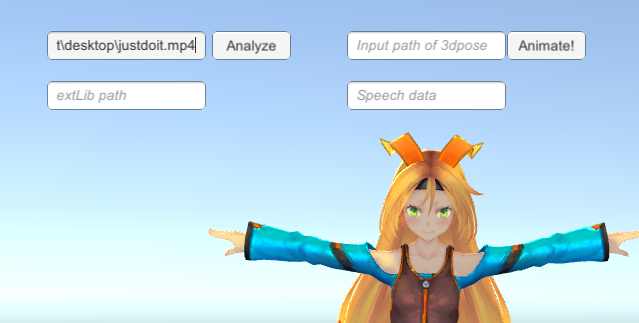
\includegraphics[width=1.0\textwidth]{fig/iw1131.png}
  %   \label{fig:iw1131}
  % \end{figure}
  %\clearpage
  \item Analyzeボタンを押すと解析が開始され,結果ファイルが出力される
  % \begin{figure}[h]
  %   \centering
  %   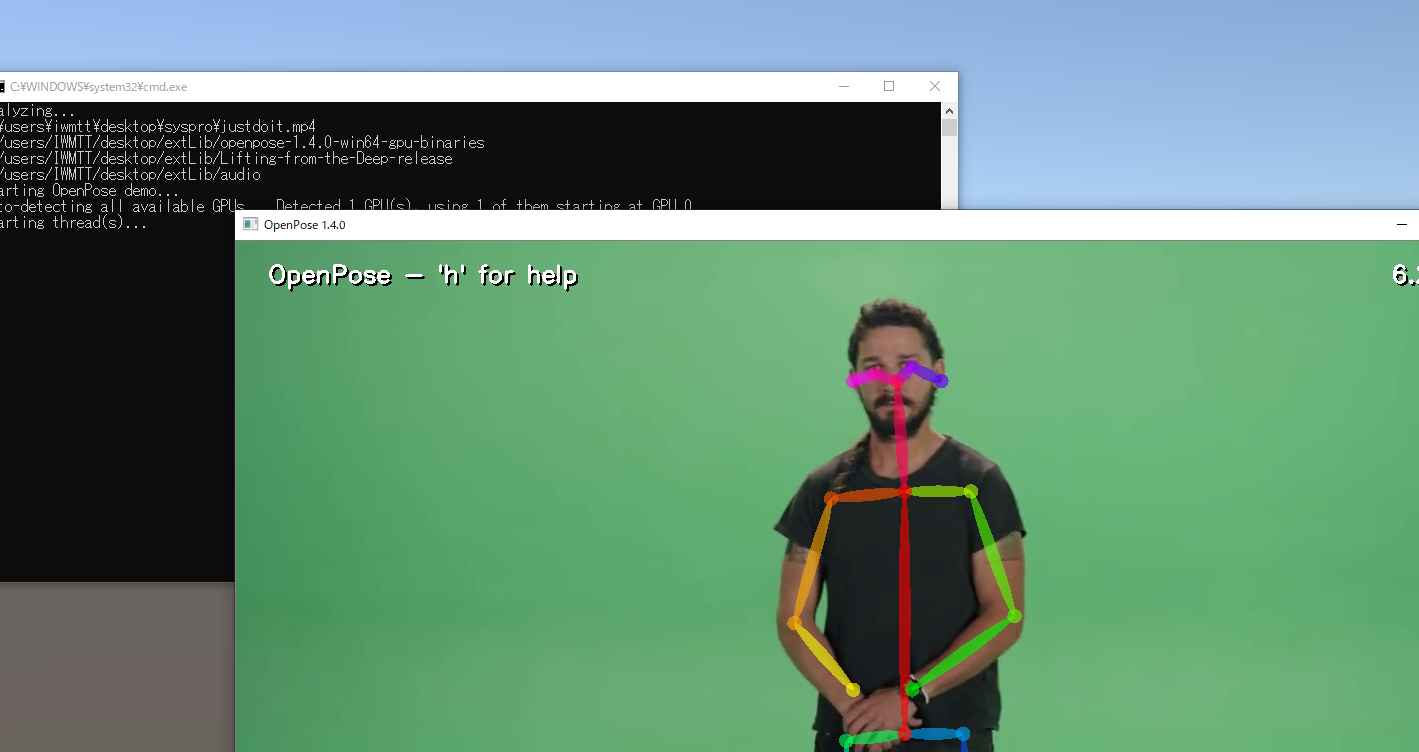
\includegraphics[width=1.0\textwidth]{fig/iw1132.png}
  %   \label{fig:iw1132}
  % \end{figure}
  \item 解析終了後Animateボタンを押すことで字幕とモデルの動きの動画が出力される.
%   \begin{figure}[h]
%     \centering
%     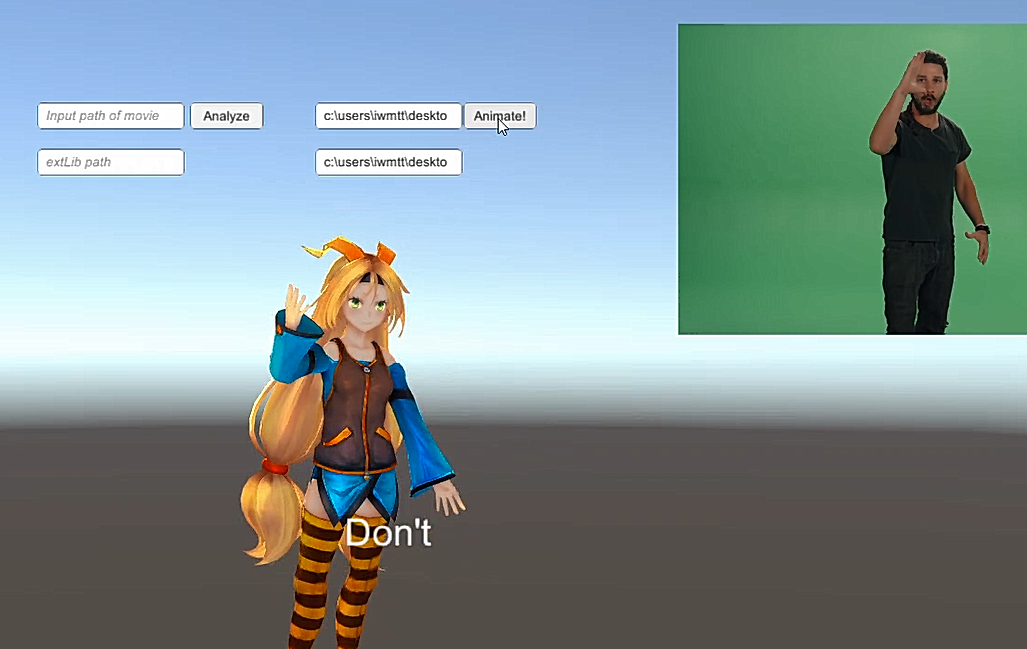
\includegraphics[width=1.0\textwidth]{fig/iw1133.png}
%     \label{fig:iw1133}
%   \end{figure}
\end{enumerate}
実際の実行の様子は同梱されたビデオファイルを参照のこと.

\begin{figure}[h]
    \centering
    \begin{tabular}{c}
      \begin{minipage}{0.3\hsize}
        \centering
        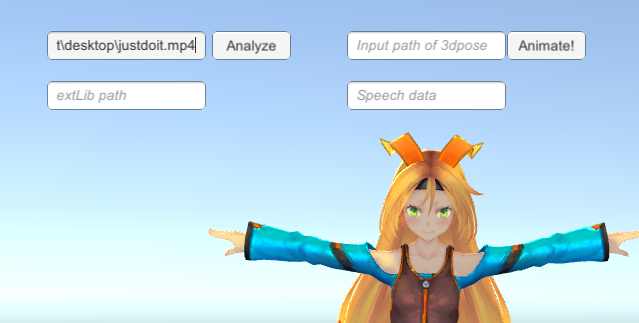
\includegraphics[width=1.0\textwidth]{fig/iw1131.png}
        \text{解析したい動画のパス指定}
      \end{minipage}

      \begin{minipage}{0.3\hsize}
        \centering
        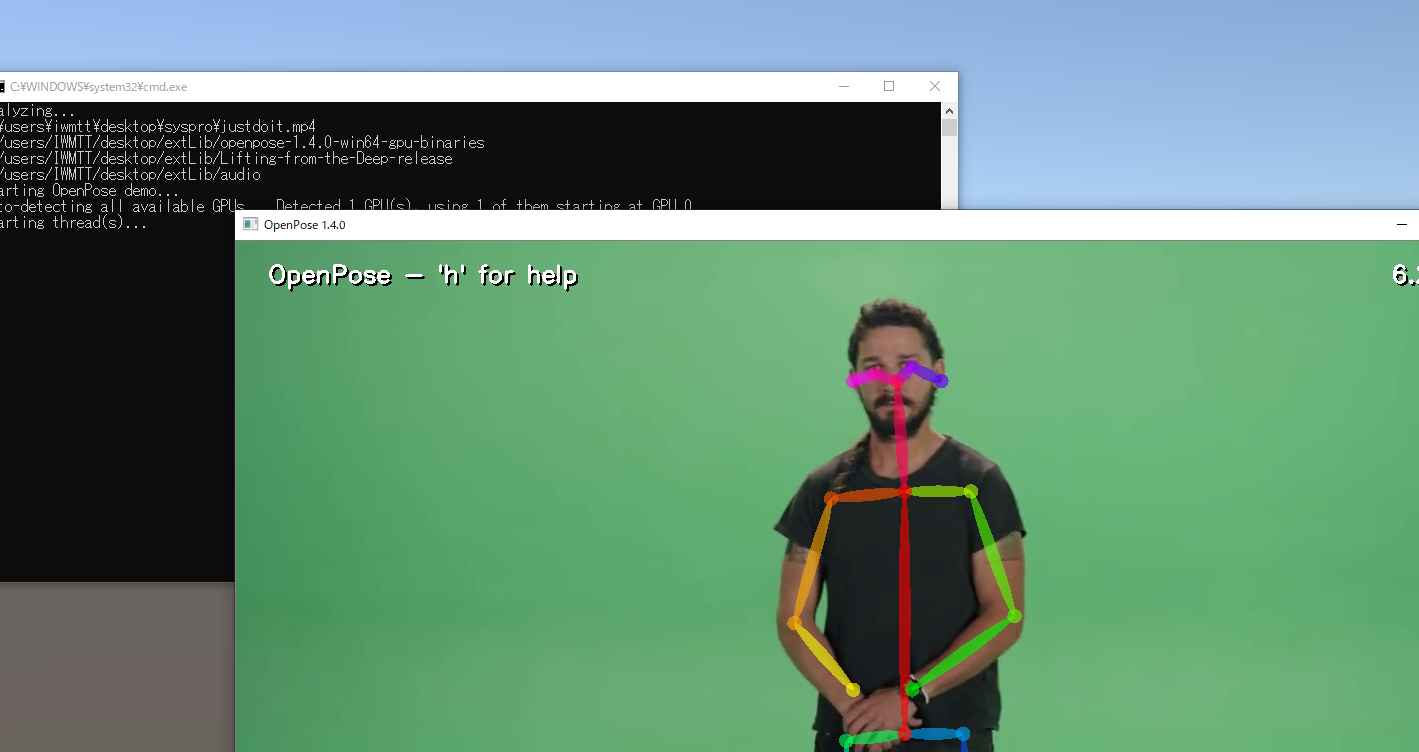
\includegraphics[width=1.0\textwidth]{fig/iw1132.png}
        \text{処理中の画面}
      \end{minipage}

      \begin{minipage}{0.3\hsize}
        \centering
        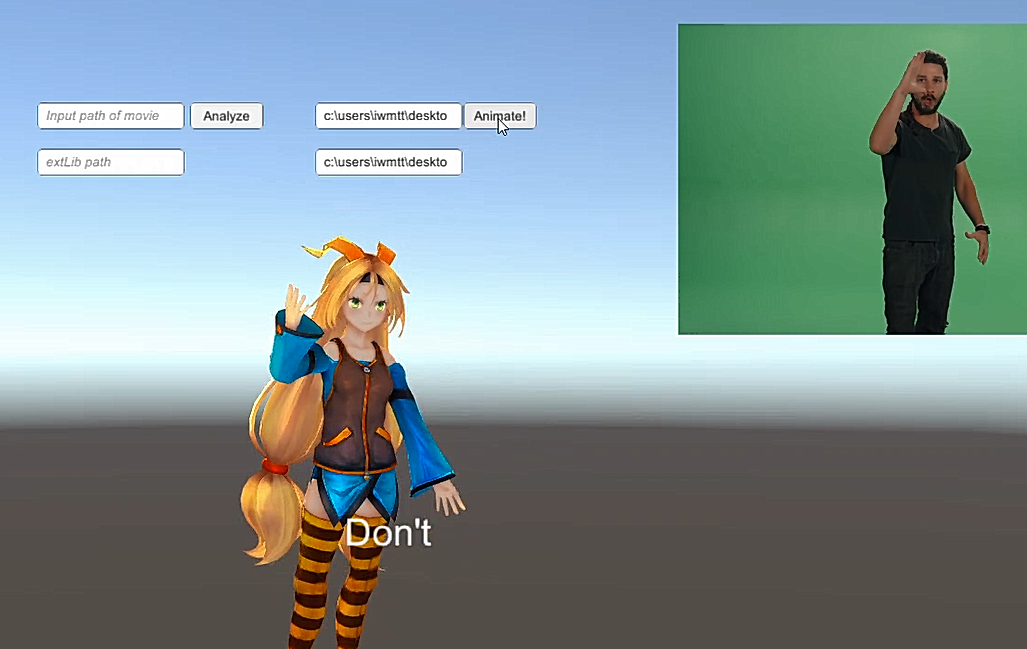
\includegraphics[width=1.0\textwidth]{fig/iw1133.png}
        \text{実行結果}
      \end{minipage}

    \end{tabular}
    \caption{ミーティング内容の比較}
    \label{fig:iw113compare}
\end{figure}





\subsection{ソフトウェアの機能・仕様}
\begin{itemize}
  \item 深度情報なしに骨格推定を行い,モデルに動きを反映させる一連の処理を画一化.
  \item 音声解析により字幕描画も実装.
  \item 推定可能人数は実装時点では1人
  \item 現時点ではUnity editor上での実行となる

\end{itemize}

\subsection{ソフトウェアの設計・製作過程}
\subsubsection{設計}
処理のフローチャートを以下の図\ref{fig:iw1311}に示す.
動画から音声などを抽出し,要素ごとに分けて処理を行っている.
通常Unityから直接pythonの仮想環境へのアクセスはできないため,今回の実装ではシェルスクリプトを介してanacondaの仮想環境にアクセスする手法をとっている.
仮想環境をセットアップするスクリプトも同梱しているため,利用者が一々必要なライブラリをインストールする必要はない.
また,専用の仮想環境を作成することで,利用者のpython環境を改変することなしに複数のライブラリの利用が可能となることも利点となる.
\begin{figure}[h]
  \centering
  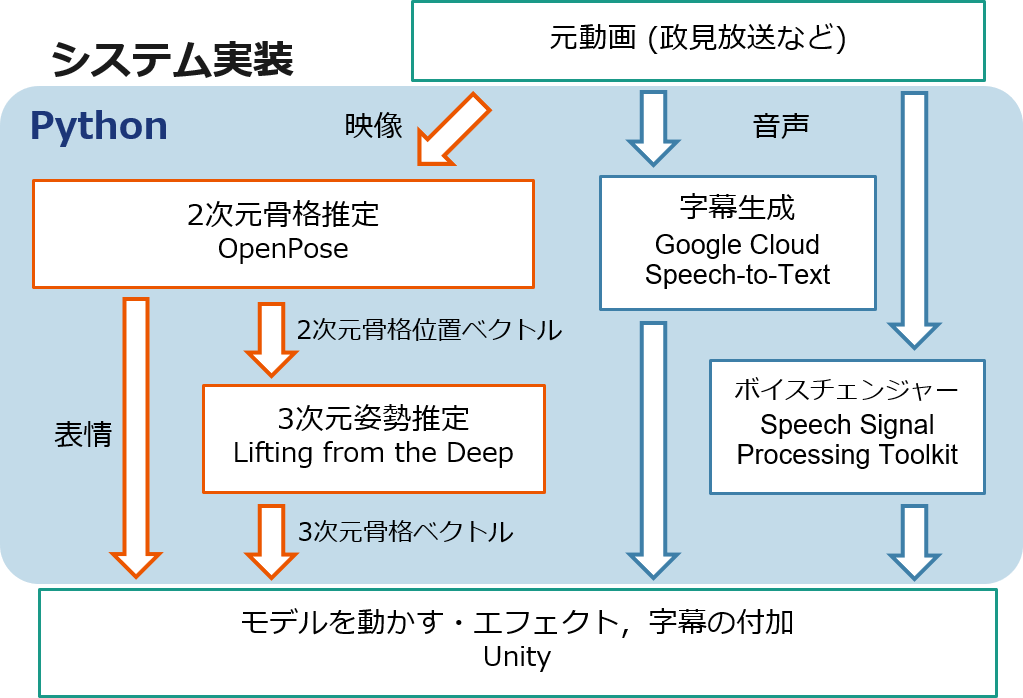
\includegraphics[width=1.0\textwidth]{fig/iw1311.png}
  \caption{処理の概要図}
  \label{fig:iw1311}
\end{figure}

\subsubsection{製作過程}
10月時点と12月時点でのミーティング事項の比較を図\ref{fig:iw132compare}に示す.
10月時点では定まっていなかった「具体的に何を使用するか」が,12月時点では明確に定まった.

\begin{figure}[h]
  \centering
 \begin{minipage}[b]{0.45\linewidth}
  \centering
  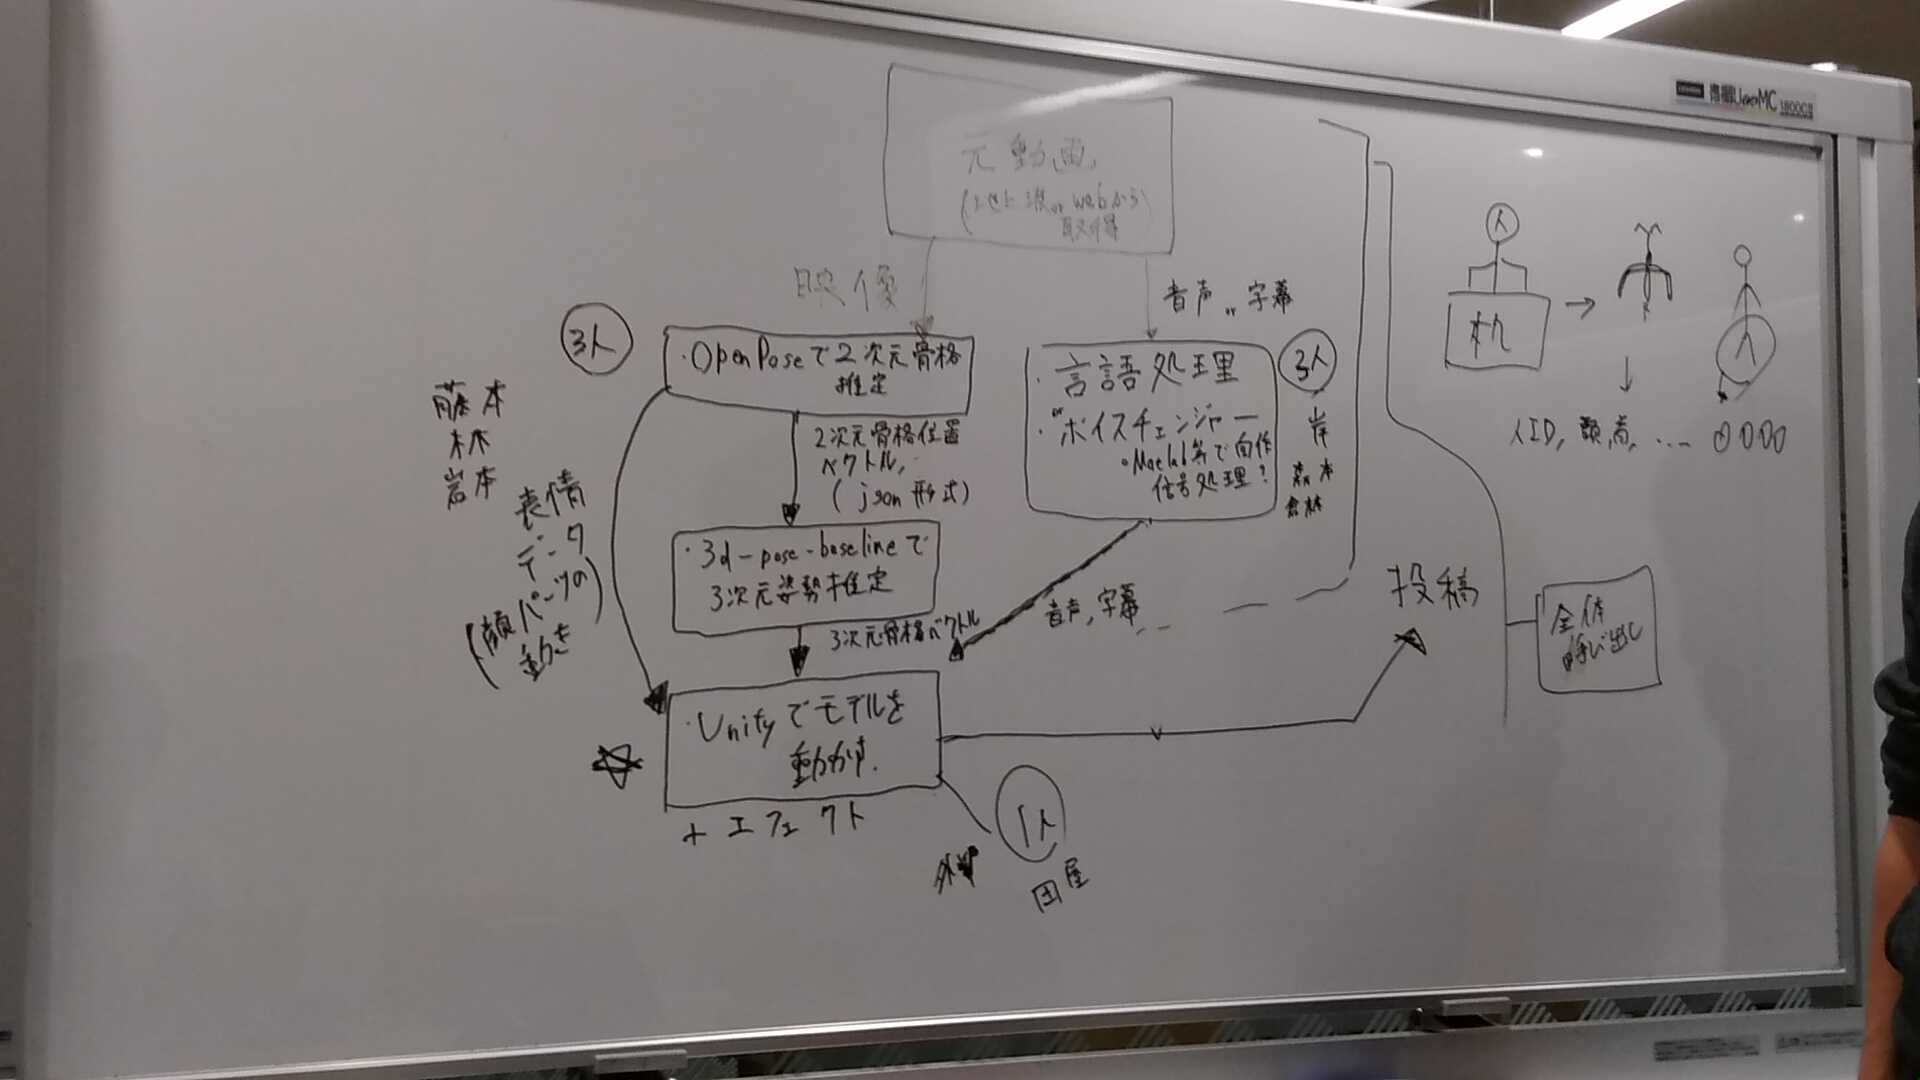
\includegraphics[width=1.0\textwidth]{fig/iw1321.png}
  \text{10月時点}
  \end{minipage}
 \begin{minipage}[b]{0.08\linewidth}
  \centering
 \end{minipage}
 \begin{minipage}[b]{0.45\linewidth}
  \centering
  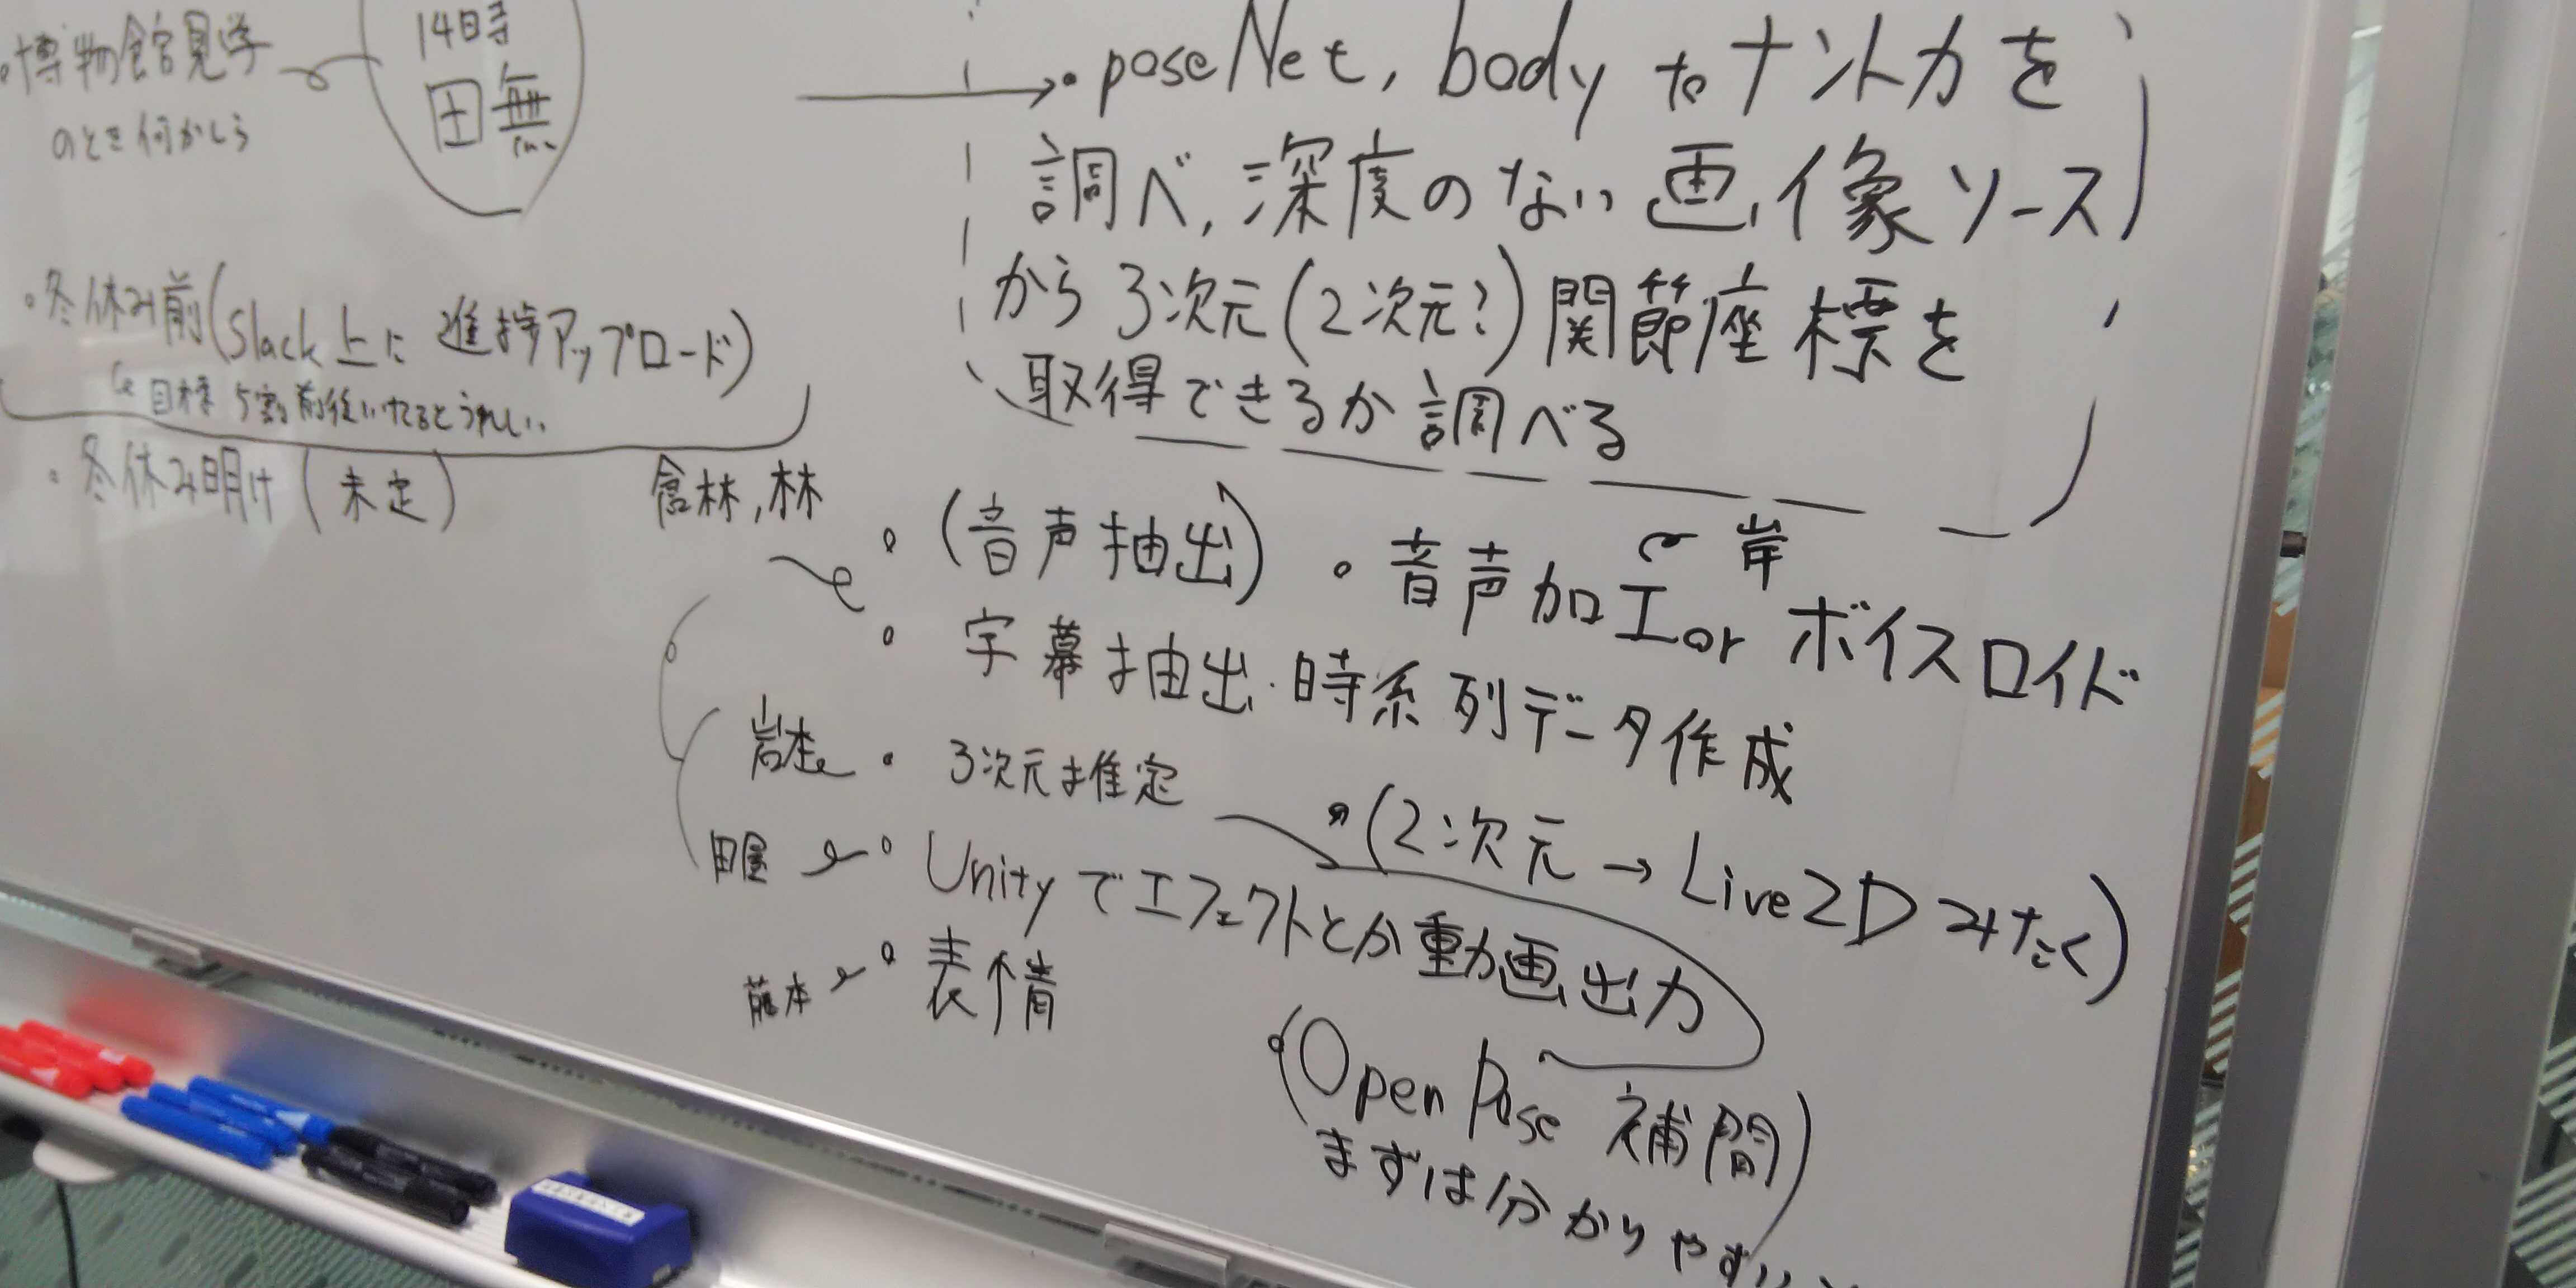
\includegraphics[width=1.0\textwidth]{fig/iw1322.png}
  \text{12月時点}
  \end{minipage}
 \caption{ミーティング内容の比較}
 \label{fig:iw132compare}
\end{figure}



\end{document}
